\documentclass[tikz,border=3.14mm]{standalone}
\usetikzlibrary{3d,positioning,arrows.meta}

\begin{document}
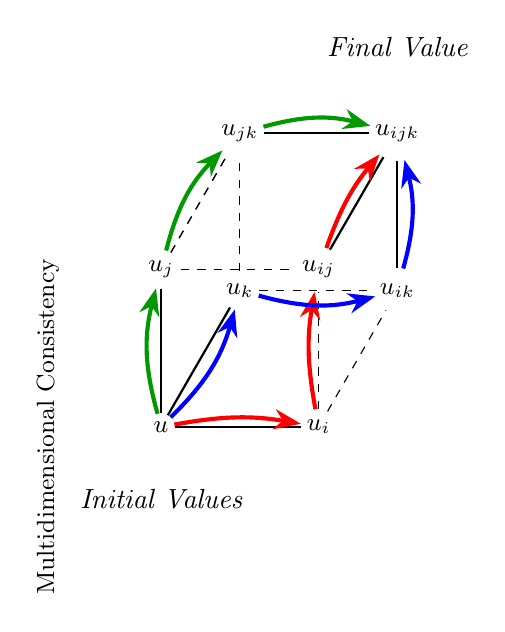
\begin{tikzpicture}[
    scale=2,
    z={(0.5,0.866)}, % Perspective projection
    back/.style={dashed, thin},
    front/.style={thick},
    path1/.style={draw=red, line width=1.5pt, -Stealth},
    path2/.style={draw=blue, line width=1.5pt, -Stealth},
    path3/.style={draw=green!60!black, line width=1.5pt, -Stealth},
    node/.style={circle, fill=white, inner sep=1pt, font=\small}
]

    % Cube vertices (bottom layer)
    \node[node] (u) at (0,0,0) {$u$};
    \node[node] (ui) at (1,0,0) {$u_i$};
    \node[node] (uj) at (0,1,0) {$u_j$};
    \node[node] (uk) at (0,0,1) {$u_k$};
    
    % Cube vertices (top layer)
    \node[node] (uij) at (1,1,0) {$u_{ij}$};
    \node[node] (uik) at (1,0,1) {$u_{ik}$};
    \node[node] (ujk) at (0,1,1) {$u_{jk}$};
    \node[node] (uijk) at (1,1,1) {$u_{ijk}$};

    % Cube edges (bottom layer)
    \draw[front] (u) -- (ui);
    \draw[front] (u) -- (uj);
    \draw[front] (u) -- (uk);
    \draw[back] (ui) -- (uij);
    \draw[back] (uj) -- (uij);
    \draw[back] (uj) -- (ujk);
    \draw[back] (uk) -- (uik);
    \draw[back] (uk) -- (ujk);
    
    % Vertical edges
    \draw[back] (ui) -- (uik);
    \draw[back] (uj) -- (ujk);
    \draw[back] (uk) -- (ujk);
    \draw[front] (uij) -- (uijk);
    \draw[front] (uik) -- (uijk);
    \draw[front] (ujk) -- (uijk);

    % Path 1: u → ui → uij → uijk (i-j plane first)
    \draw[path1] (u) to[bend left=10] (ui);
    \draw[path1] (ui) to[bend left=10] (uij);
    \draw[path1] (uij) to[bend left=10] (uijk);

    % Path 2: u → uk → uik → uijk (i-k plane first)
    \draw[path2] (u) to[bend right=15] (uk);
    \draw[path2] (uk) to[bend right=15] (uik);
    \draw[path2] (uik) to[bend right=15] (uijk);

    % Path 3: u → uj → ujk → uijk (j-k plane first)
    \draw[path3] (u) to[bend left=15] (uj);
    \draw[path3] (uj) to[bend left=15] (ujk);
    \draw[path3] (ujk) to[bend left=15] (uijk);

    % Annotations
    \node[below=5mm of u, anchor=north, font=\itshape] {Initial Values};
    \node[above=5mm of uijk, anchor=south, font=\itshape] {Final Value};
    \node[left=1cm of u, rotate=90, anchor=south, font=\small] {Multidimensional Consistency};
\end{tikzpicture}
\end{document}